\documentclass[11pt]{article}

\usepackage{texyousei}
\usepackage{tabularx}

\lhead{}
\chead{}
\rhead{}

\usepackage{comment}
\excludecomment{oops}

\setlength{\leftmargini}{0.3in}

\DeclarePairedDelimiter{\inner}{\langle}{\rangle}
\newcommand{\ddx}{\frac{d}{dx}}
\newcommand{\ddy}{\frac{d}{dy}}
\newcommand{\ddn}{\frac{d}{dn}}
\newcommand{\ddm}{\frac{d}{dm}}
\newcommand{\sgn}[1]{\ \textrm{sgn}\left(#1\right)}
\newcommand{\calDf}{\mathcal{D}_f}

\begin{document}

\maketitle{Path Planning using Repulsive Energies}{Chris Yu (christoy@cs.cmu.edu)}

\thispagestyle{empty}

\begin{figure}[h]
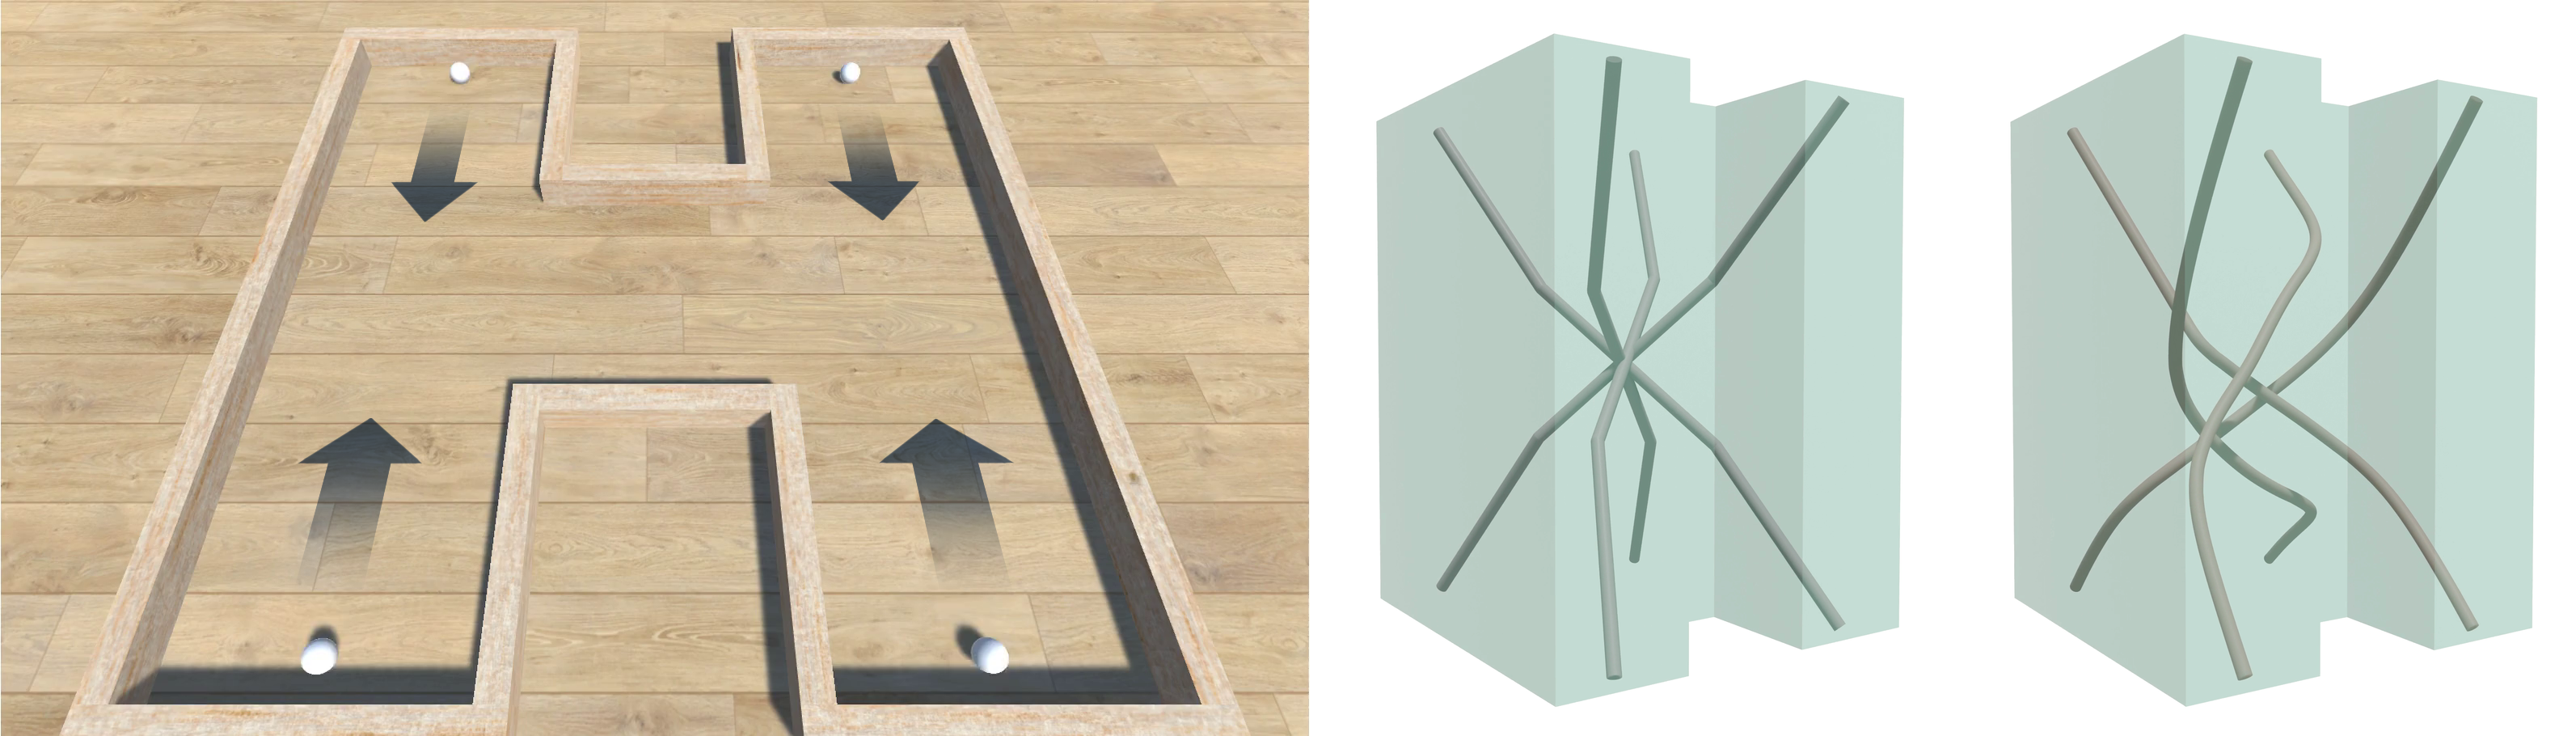
\includegraphics[width=\textwidth]{pathplan.png}
\caption{\emph{Left:} A path planning scenario in which each agent must move to the opposite corner. \emph{Right:} Motion trajectories can be represented as 3D curves, which can be optimized.}
\end{figure}

\paragraph{Background and motivation.} Avoiding collisions and self-collisions is a frequent challenge in design tasks. \emph{Repulsive energy functions} can be used to facilitate self-avoidance on curves and surfaces; these energies present an infinite potential barrier to collisions, and their gradient flows thus repel shapes, preventing them from self-intersecting.

One potential application of these energies lies in path planning, either involving single or multiple agents. Consider a robot that travels along the ground; its environment can be represented as a planar 2-dimensional region. Suppose that the robot's goal is to travel from point $x$ of its environment to point $y$. This equates to finding a time-parameterized curve $\gamma : [0,1] \to \R^2$ connecting the two points, meaning $\gamma(0) = x$ and $\gamma(1) = y$. The 3-dimensional graph of this curve then corresponds to a space curve in $\R^2 \times [0,1] \subset \R^3$, where the third coordinate corresponds to time. This curve can be optimized using repulsive energies to be made more robust to collisions.

The problem becomes even more interesting when multiple agents are involved; each agent's trajectory then corresponds to a separate curve $\gamma_i \subset \R^2 \times [0,1]$, and in addition to each such curve avoiding obstacles, the curves must also avoid each other -- a task that repulsive energies are well-suited for.

\paragraph{Goals.} The goal will be to develop a practical path planning algorithm for 2D environments, involving either single agents or multiple agents, that combines traditional approaches (e.g. traditional graph search) with continuous optimization using repulsive energies. The continuous optimization aspect of the problem so far does not seem to have been well-explored so far in path planning literature.

\paragraph{Skill set.} Students should ideally be familiar with basic differential geometry related to curves in space, as well as introductory optimization concepts such as gradient descent. Programming experience with C++ is also desirable. Some familiarity with robotic path planning is a bonus.



\end{document}

